\myparagraph{Le nano ordinateur}
\begin{figure}[H]
    \centering
    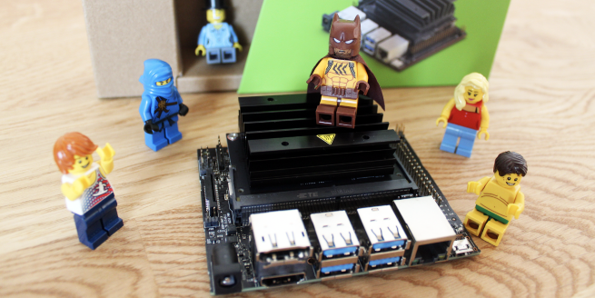
\includegraphics[width=1.0\textwidth]{jetson_nano_lego}
    \caption[Carte mère Jetson Nano de NVIDIA]{Carte mère Jetson Nano de NVIDIA, représenté avec des Lego pour démontrer sa petitesse}
    \label{fig:jetson_nano_lego}
\end{figure}
\par L'objet d'étude de cet essai est un nano ordinateur. Un nano ordinateur est un ordinateur miniaturisé en taille, mais aussi limité en capacité. Il existe différents fabricants et modèles, de caractéristiques techniques variées, pour répondre à différents besoins. Le dernier né est le modèle "Jetson nano" du fabricant "NVIDIA" (figure \ref{fig:jetson_nano_lego}), disponible depuis juin 2019 au prix très abordable de 99\$US. La compagnie NVIDIA a conçu ce matériel spécialement pour différentes applications d'inférence de modèles d'apprentissage profond sur une plateforme mobile (drone) ou proche des données ("edge" en anglais). Ce modèle a été choisi afin de répondre à l'intérêt que suscitent ses capacités et ses limites. 
\myparagraph{Logiciels}
\par De même que pour les périphériques, les solutions logiciels principales qui seront utilisés dans le cadre de l'essai sont résumés dans le tableau suivant, où il est indiqué leur nom, le type de licence, leur version, leurs rôles et responsabilités, comme pour le système d'exploitation, l'environnement de développement pour l'apprentissage profond, l'inférence, les logiciels de traitements vidéos et d'images. 
\par Pour tester les performances de la micro-sd et du disque SDD interne M.2 NVMe, l'utilitaire "hdparm" a été utilisé. Il est nécessaire de l'installer (`sudo apt-get install hdparm`) car il n'est pas inclus de base avec le système L4T.
\par Le SDK qui sera utilisé avec le nano ordinateur sera celui fourni par NVIDIA et qui se nomme "JetPack"\footnote{\url{https://developer.nvidia.com/embedded/jetpack}} \footnote{\url{https://docs.nvidia.com/jetson/jetpack/introduction/index.html}}. La version 4.4\footnote{\url{https://developer.nvidia.com/embedded/jetpack-archive}} sera celle avec laquelle les tests de performance ont été exeécuté. Il contient le système d'exploitation Linux For Tegra (L4T)\footnote{\url{https://developer.nvidia.com/embedded/linux-tegra}} (version L4T 32.4.3), qui est une version de la distribution Linux Ubuntu 18.04 mise à la saveur de NVIDIA. Jetpack contient aussi d'autres librairies qui sont nécessaires pour l'inférence, tel que Cuda, CuDn et TensorRT.
\begin{figure}[H]
    \centering
    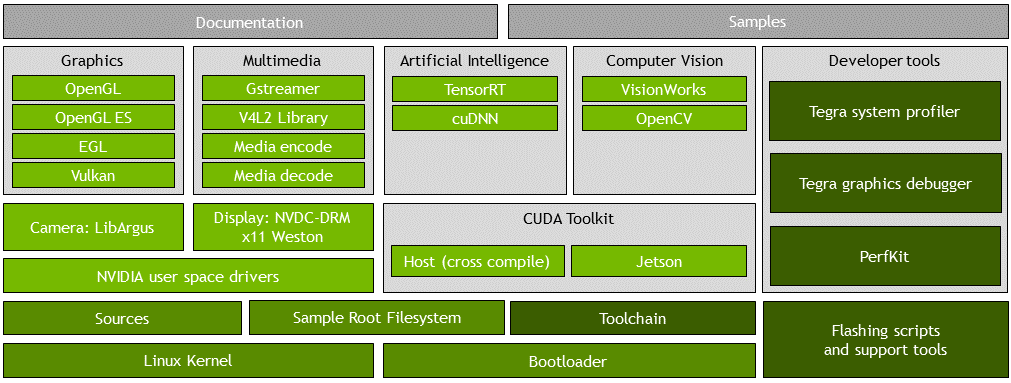
\includegraphics[width=1.0\textwidth]{jetpack_architecture}
    \caption[Diagramme de l'architecture du NVIDIA JetPack]{Diagramme de l'architecture du NVIDIA JetPack\protect\footnotemark}
    \label{fig:jetpack_architecture}
\end{figure}
\footnotetext{\url{https://docs.nvidia.com/jetson/l4t/index.html#page/Tegra\%2520Linux\%2520Driver\%2520Package\%2520Development\%2520Guide\%2Foverview.html\%23}}
\par Python et le C++ sont les languages utilisés par le framework de DeepLearning de NVIDIA. Python est utilisé comme language accessible et appelle les extensions écritent en C++ et qui optimisent les accès aux ressources systèmes tel que les CPUs et GPUS, les traitement des images et vidéos, les boucles et les traitements mémoires intensifs.
\par La librairie d’apprentissage profond qui sera utilisée est PyTorch, bonifié avec une version adaptée par NVIDIA de torchvision, qui fournie des modèles d'architecture et des utilitaires pour la vision par ordinateur (computer vision). Des versions bien spécifiques sont nécessaires et il est important de s'y conformer au risque de tomber dans une investigation bien coûteuse en temps et énergie\footnote{\url{https://forums.developer.nvidia.com/t/trying-to-regenerate-onnx-for-jetson-nano/125494?u=vincelf}}.
\par Le nano ordinateur inclut un GPU qui est mis à contribution lors de l'inférence. Le compilateur de NVIDIA pour GPU 'cuda' est nécessaire pour regénérer le .onnx lors de la phase d'adaption. La version doit concorder avec la bonne version de PyTorch. La version adaptée (fork) de torchvision doit être recompilée avec la bonne version de pytorch et cuda. 
\par Enfin pour régénérer le .onnx lors de la phase d'adaptation, les librairies TensorRT et ONNX ont été utilisées, en compagnie de l'utilitaire `trtexec` qui permet de valider et tester le fichier .onnx généré.
\par Lors de la phase d'évaluation des performances systèmes, les utilitaires tegrastats, free, iotop ont été utilisés.
{
    \vspace{0.3em} % Adjust the height of the space between caption and tabular
    \begin{longtable}[t]{{@{}|p{5em}|p{3em}|p{3em}|p{24em}|@{}}} % p{15em}p{35em} with landscape
        \caption{Solutions logicielles de l'essai}\label{table:table_sol_logiciel}\\
        \hline
        \textbf{Language} & \textbf{Version} & \textbf{Licence} & \textbf{Rôles et responsabilités} \\
        \endfirsthead
        \hline
        \textbf{Language} & \textbf{Version} & \textbf{Licence} & \textbf{Rôles et responsabilités} \\
        \hline
        \endhead
        \endfoot
        \endlastfoot
        \hline
        JetpPack & 4.4 & NVIDIA & Kit de développement de logiciels incluant le système d'exploitation L4T, et les librairies et utilitaires nécessaires pour l'inférence avec le nano ordinateur.\\
        \hline
        L4T & 32.4.3 & NVIDIA & Le sytème d'exploitation "Linux For Tegra" conçut par NVIDIA pour leurs solutions d'inférence légères, comme pour le nano ordinateur.\\
        \hline
        Python & 2.7 & GPL & Language plus accessible que le C++.\\
        \hline
        C++ & GCC 7.3.1\footnote{\url{https://developer.nvidia.com/embedded/linux-tegra}} & GPL & Certaines extensions du cadre applicatif de NVIDIA pour l'inférence sont écrites en C++, pour des raisons d'optimisation.\\
        \hline
        pytorch & 1.1.0 & BSD 3-Clause & Cadres d'application logicielle ("framework") pour l'apprentissage machine et profond.\\
        \hline
        torchvision & & BSD 3-Clause & Branche de torchvision adaptée par NVIDIA\footnote{\url{https://github.com/dusty-nv/vision.git} et ensuite branche v0.3.0}; Doit être recompilée avec la version de pytorch 1.1.0 et cuda 10.0.\\
        \hline
        cuda & 10.0 & NVIDIA & Compilateur de code C++ pour GPU.\\
        \hline
        TensorRT & 6.0.1.5 & NVIDIA & Librairies pour générer des modèles optimisés pour l'inférence.\\
        \hline
        ONNX & & MIT & Permet lde générer un format interopérable pour l'inférence de modèles d'architecture construit avec différent framework de machine learning (Caffe, PyTorch, TensorFlow, etc).\\
        \hline
        trtexec & & NVIDIA & Utilitaire qui a permis de tester le .onnx qui a été regénéré.\\
        \hline
        gstreamer & 1.1 & LGPL & Utilitaire qui a permis d'alimenter le modèle de la segmentation avec la vidéo.\\
        \hline
        v4l2loopback & & GPL & Utilitaire qui a permis de créer un matériel vidéo virtuelle permettant de remplaçer la caméra, permettant ainsi au modèle d'être alimenté par une vidéo et non la caméra.\\
        \hline
        hdparm & & GPL & Utilitaire permettant de tester la capacité de lecture d'une unité de stockage, tel que'un SSD NVMe et différentes cartes micro-sd.\\
        \hline
        tegrastats & & NVIDIA & La commande offre différents indicateurs système tel que l'utilisation des processeurs, la température, la consommation, et qui sont utiles pour observer le comportement du système lors des tests de performance de la segmentation.\\
        \hline
        free & & GPL & La commande offre le status de la mémoire totale, utilisée, libre, swap, cachée, etc. Elle est utile pour observer le comportement de la mémoire du nano ordinateur lors des tests de performance de la segmentation.\\
        \hline
        iotop & & GPL & La commande offre le status des opérations "I/O" de lecture \& écriture sur le disque, totale ou pour le processus de segmentation. Elle est utile pour observer le comportement des opérations sur le disque du nano ordinateur lors des tests de performance de la segmentation.\\
        \hline
    \end{longtable}
}
% {
%     \renewcommand*{\arraystretch}{1.4}
%     \begin{table}[htb]
%         \centering
%         \caption{Solutions logicielles de l'essai}\label{table:table_sol_logiciel}
%         \vspace{0.3em} % Adjust the height of the space between caption and tabular
%         \begin{tabular}{{@{}|p{5em}|p{3em}|p{3em}|p{24em}|@{}}}
%         % \begin{tabular}{|c|c|c|} % does not work don't know why
%             \hline
%             \textbf{Language} & \textbf{Version} & \textbf{Licence} & \textbf{Rôles et responsabilités} \\
%             \hline
%             JetpPack & 4.4 & NVIDIA & Kit de développement de logiciels incluant le système d'exploitation L4T, et les librairies et utilitaires nécessaires pour l'inférence avec le nano ordinateur.\\
%             \hline
%             L4T & 32.4.3 & NVIDIA & Le sytème d'exploitation "Linux For Tegra" conçut par NVIDIA pour leurs solutions d'inférence légères, comme pour le nano ordinateur.\\
%             \hline
%             Python & 2.7 & GPL & Language plus accessible que le C++.\\
%             \hline
%             C++ & GCC 7.3.1\footnote{\url{https://developer.nvidia.com/embedded/linux-tegra}} & GPL & Certaines extensions du cadre applicatif de NVIDIA pour l'inférence sont écrites en C++, pour des raisons d'optimisation.\\
%             \hline
%             pytorch & 1.1.0 & BSD 3-Clause & Cadres d'application logicielle ("framework") pour l'apprentissage machine et profond.\\
%             \hline
%             torchvision & & BSD 3-Clause & Branche de torchvision adaptée par NVIDIA\footnote{\url{https://github.com/dusty-nv/vision.git} et ensuite branche v0.3.0}; Doit être recompilée avec la version de pytorch 1.1.0 et cuda 10.0.\\
%             \hline
%             cuda & 10.0 & NVIDIA & Compilateur de code C++ pour GPU.\\
%             \hline
%             TensorRT & 6.0.1.5 & NVIDIA & Librairies pour générer des modèles optimisés pour l'inférence.\\
%             \hline
%             ONNX & & MIT & Permet lde générer un format interopérable pour l'inférence de modèles d'architecture construit avec différent framework de machine learning (Caffe, PyTorch, TensorFlow, etc).\\
%             \hline
%             trtexec & & NVIDIA & Utilitaire qui a permis de tester le .onnx qui a été regénéré.\\
%             \hline
%             gstreamer & 1.1 & LGPL & Utilitaire qui a permis d'alimenter le modèle de la segmentation avec la vidéo.\\
%             \hline
%             v4l2loopback & & GPL & Utilitaire qui a permis de créer un matériel vidéo virtuelle permettant de remplaçer la caméra, permettant ainsi au modèle d'être alimenté par une vidéo et non la caméra.\\
%             \hline
%             hdparm & & GPL & Utilitaire permettant de tester la capacité de lecture d'une unité de stockage, tel que'un SSD NVMe et différentes cartes micro-sd.\\
%             \hline
%             tegrastats & & NVIDIA & La commande offre différents indicateurs système tel que l'utilisation des processeurs, la température, la consommation, et qui sont utiles pour observer le comportement du système lors des tests de performance de la segmentation.\\
%             \hline
%             free & & GPL & La commande offre le status de la mémoire totale, utilisée, libre, swap, cachée, etc. Elle est utile pour observer le comportement de la mémoire du nano ordinateur lors des tests de performance de la segmentation.\\
%             \hline
%             iotop & & GPL & La commande offre le status des opérations "I/O" de lecture \& écriture sur le disque, totale ou pour le processus de segmentation. Elle est utile pour observer le comportement des opérations sur le disque du nano ordinateur lors des tests de performance de la segmentation.\\
%             \hline
%         \end{tabular}
%     \end{table}
% }
\clearpage
\newpage